\documentclass[aspectratio=169]{ctexbeamer}
% \setbeamertemplate{bibliography item}{\insertbiblabel}
\usepackage{booktabs}
\usepackage{listings}
\usepackage{xcolor}
\usepackage{float}
\usetheme{Madrid}

\title{Auto-Vectorization \& SIMD in LLVM}
\subtitle{High Performance Computing}

\AtBeginSection[]{
    \begin{frame}
        \vfill
        \centering
        \begin{beamercolorbox}[sep=8pt,center,shadow=true,rounded=true]{title}
            \usebeamerfont{title}\insertsectionhead\par%
        \end{beamercolorbox}
        \vfill
    \end{frame}
}

\beamertemplatenavigationsymbolsempty
\definecolor{tuna}{rgb}{0.098,0.51,0.696}
\definecolor{thu}{rgb}{0.50,0.36,0.71}

\setbeamercolor{section in toc}{fg=black,bg=white}
\setbeamercolor{item}{fg=tuna,bg=white}
\setbeamercolor{alerted text}{fg=tuna!80!gray}
\setbeamercolor*{palette primary}{fg=tuna!60!black,bg=gray!30!white}
\setbeamercolor*{palette secondary}{fg=tuna!70!black,bg=gray!15!white}
\setbeamercolor*{palette tertiary}{bg=tuna!80!black,fg=gray!10!white}
\setbeamercolor*{palette quaternary}{fg=tuna,bg=gray!5!white}

\setbeamercolor*{sidebar}{fg=tuna,bg=gray!15!white}

\setbeamercolor*{palette sidebar primary}{fg=tuna!10!black}
\setbeamercolor*{palette sidebar secondary}{fg=white}
\setbeamercolor*{palette sidebar tertiary}{fg=tuna!50!black}
\setbeamercolor*{palette sidebar quaternary}{fg=gray!10!white}

%\setbeamercolor*{titlelike}{parent=palette primary}
\setbeamercolor{titlelike}{parent=palette primary,fg=tuna}
\setbeamercolor{frametitle}{bg=gray!10!white}
\setbeamercolor{frametitle right}{bg=gray!60!white}

\setbeamercolor*{separation line}{}
\setbeamercolor*{fine separation line}{}

\setbeamertemplate{sections/subsections in toc}[square]
\setbeamertemplate{items}[square]

% define some basic colors
\definecolor{mauve}{rgb}{0.58,0,0.82}

\definecolor{codegreen}{rgb}{0,0.6,0}
\definecolor{codegray}{rgb}{0.5,0.5,0.5}
\definecolor{codepurple}{rgb}{0.58,0,0.82}
\definecolor{backcolour}{rgb}{1,1,1}


\setmonofont{Consolas}

\lstset{
% listings sonderzeichen (for german weirdness)
literate={ö}{{\"o}}1
{ä}{{\"a}}1
{ü}{{\"u}}1,
basicstyle=\tiny\ttfamily,                    % very small code
breaklines=true,                              % break long lines
commentstyle=\itshape\color{green!50!black},  % comments are green
keywordstyle=[1]\color{blue!80!black},        % instructions are blue
keywordstyle=[2]\color{orange!80!black},      % sections/other directives are orange
keywordstyle=[3]\color{red!50!black},         % registers are red
stringstyle=\color{mauve},                    % strings are from the telekom
identifierstyle=\color{teal},                 % user declared addresses are teal
frame=l,                                      % black line on the left side of code
language=C++,                   % all code is RISC-V
tabsize=4,                                    % indent tabs with 4 spaces
showstringspaces=false                        % do not replace spaces with weird underlines
}

\lstdefinestyle{mystyle}
{
    backgroundcolor=\color{backcolour},
    commentstyle=\color{codegreen},
    keywordstyle=\color{magenta},
    numberstyle=\tiny\color{codegray},
    stringstyle=\color{codepurple},
    basicstyle=\ttfamily\footnotesize,
    breakatwhitespace=false,
    breaklines=true,
    captionpos=b,
    keepspaces=true,
    numbers=none,
    numbersep=5pt,
    showspaces=false,
    showstringspaces=false,
    showtabs=false,
    tabsize=2,
    frame=none
}

\lstset{style=mystyle,language=C++}

\lstdefinelanguage[RISC-V]{Assembler}
{
    alsoletter={.}, % allow dots in keywords
    alsodigit={0x}, % hex numbers are numbers too!
    morekeywords=[1]{ % instructions
            lb, lh, lw, lbu, lhu,
            sb, sh, sw,
            sll, slli, srl, srli, sra, srai,
            add, addi, sub, lui, auipc,
            xor, xori, or, ori, and, andi,
            slt, slti, sltu, sltiu,
            beq, bne, blt, bge, bltu, bgeu,
            j, jr, jal, jalr, ret,
            scall, break, nop
        },
    morekeywords=[2]{ % sections of our code and other directives
            .align, .ascii, .asciiz, .byte, .data, .double, .extern,
            .float, .globl, .half, .kdata, .ktext, .set, .space, .text, .word
        },
    morekeywords=[3]{ % registers
            zero, ra, sp, gp, tp, s0, fp,
            t0, t1, t2, t3, t4, t5, t6,
            s1, s2, s3, s4, s5, s6, s7, s8, s9, s10, s11,
            a0, a1, a2, a3, a4, a5, a6, a7,
            ft0, ft1, ft2, ft3, ft4, ft5, ft6, ft7,
            fs0, fs1, fs2, fs3, fs4, fs5, fs6, fs7, fs8, fs9, fs10, fs11,
            fa0, fa1, fa2, fa3, fa4, fa5, fa6, fa7
        },
    morecomment=[l]{;},   % mark ; as line comment start
    morecomment=[l]{\#},  % as well as # (even though it is unconventional)
    morestring=[b]",      % mark " as string start/end
    morestring=[b]'       % also mark ' as string start/end
}

\author{Y.C. Long}



\begin{document}

\begin{frame}
    \maketitle
\end{frame}

\begin{frame}
    \frametitle{Table of Contents}

    \tableofcontents

\end{frame}

\section{Moore定律的终结和并行化的需求}

\begin{frame}
    \frametitle{Moore's Law to be over}

    集成电路上可容纳的晶体管数目,约每隔两年便会增加一倍

    \begin{figure}[h]
        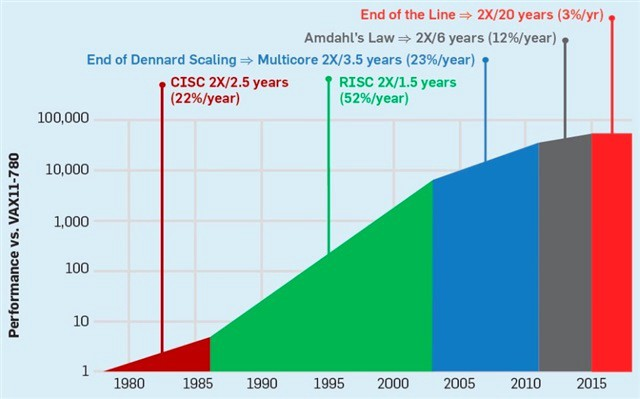
\includegraphics[height=0.5\textheight]{images/moore.jpeg}
        \caption{Moore's Law}
    \end{figure}

\end{frame}

\begin{frame}
    \frametitle{Parallel}

    提高计算机性能的方法,是并行化。

    \begin{figure}[h]
        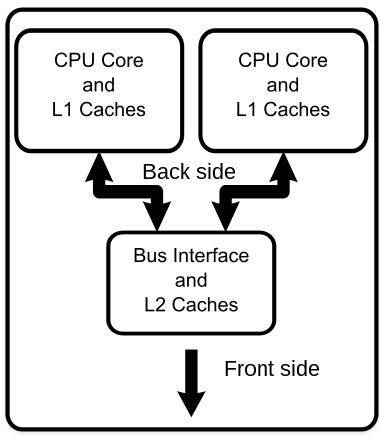
\includegraphics[height=0.5\textheight]{images/dual_core.png}
        \caption{Dual Core Cache Design}
    \end{figure}

\end{frame}

\section{并行的手段}

\subsection{Multi-Core}

\begin{frame}
    \frametitle{Multi-Core}

    为了实现并行化,我们可以给一个计算机加入多个核心。

    \begin{itemize}
        \item 不同的寄存器
        \item 不同的中断处理请求
        \item 操作系统-对称多处理(SMP)调度
    \end{itemize}

    \begin{figure}[h]
        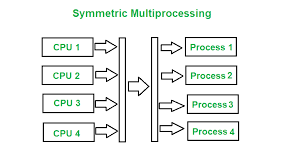
\includegraphics[height=0.45\textheight]{images/smp.png}
        \caption{Symmetric multiprocessing}
    \end{figure}

\end{frame}

\subsection{Single-Core}

\begin{frame}[fragile]
    \frametitle{Single-Core - Out-of-Order Execution}

    乱序执行(Out-of-Order Execution)是现代CPU最基本的一个并行手段。
    \begin{minipage}[t]{0.45\linewidth}
        \begin{lstlisting}[language=C++]
int test(int &a,
         int &b,
         int &c,
         int &d) {
    a += b;
    c += d;
    return 0;
}
        \end{lstlisting}
    \end{minipage}
    \begin{minipage}[t]{0.45\linewidth}
        \begin{lstlisting}[language={[RISC-V]Assembler}]
    lw      a1, 0(a1)
    lw      a4, 0(a0)
    addw    a1, a1, a4
    sw      a1, 0(a0)
    lw      a0, 0(a3)
    lw      a1, 0(a2)
    addw    a0, a0, a1
    sw      a0, 0(a2)
        \end{lstlisting}
    \end{minipage}


\end{frame}

\begin{frame}
    \frametitle{Single-Core - SIMD}

    OoOE在编程上由编译器全局指令调度器(Instruction Scheduler)优化。

    单指令流多数据流(Single instruction, multiple data (SIMD)),提供了一种让我
    们更好地进行向量计算的方式。

    \begin{figure}
        \centering
        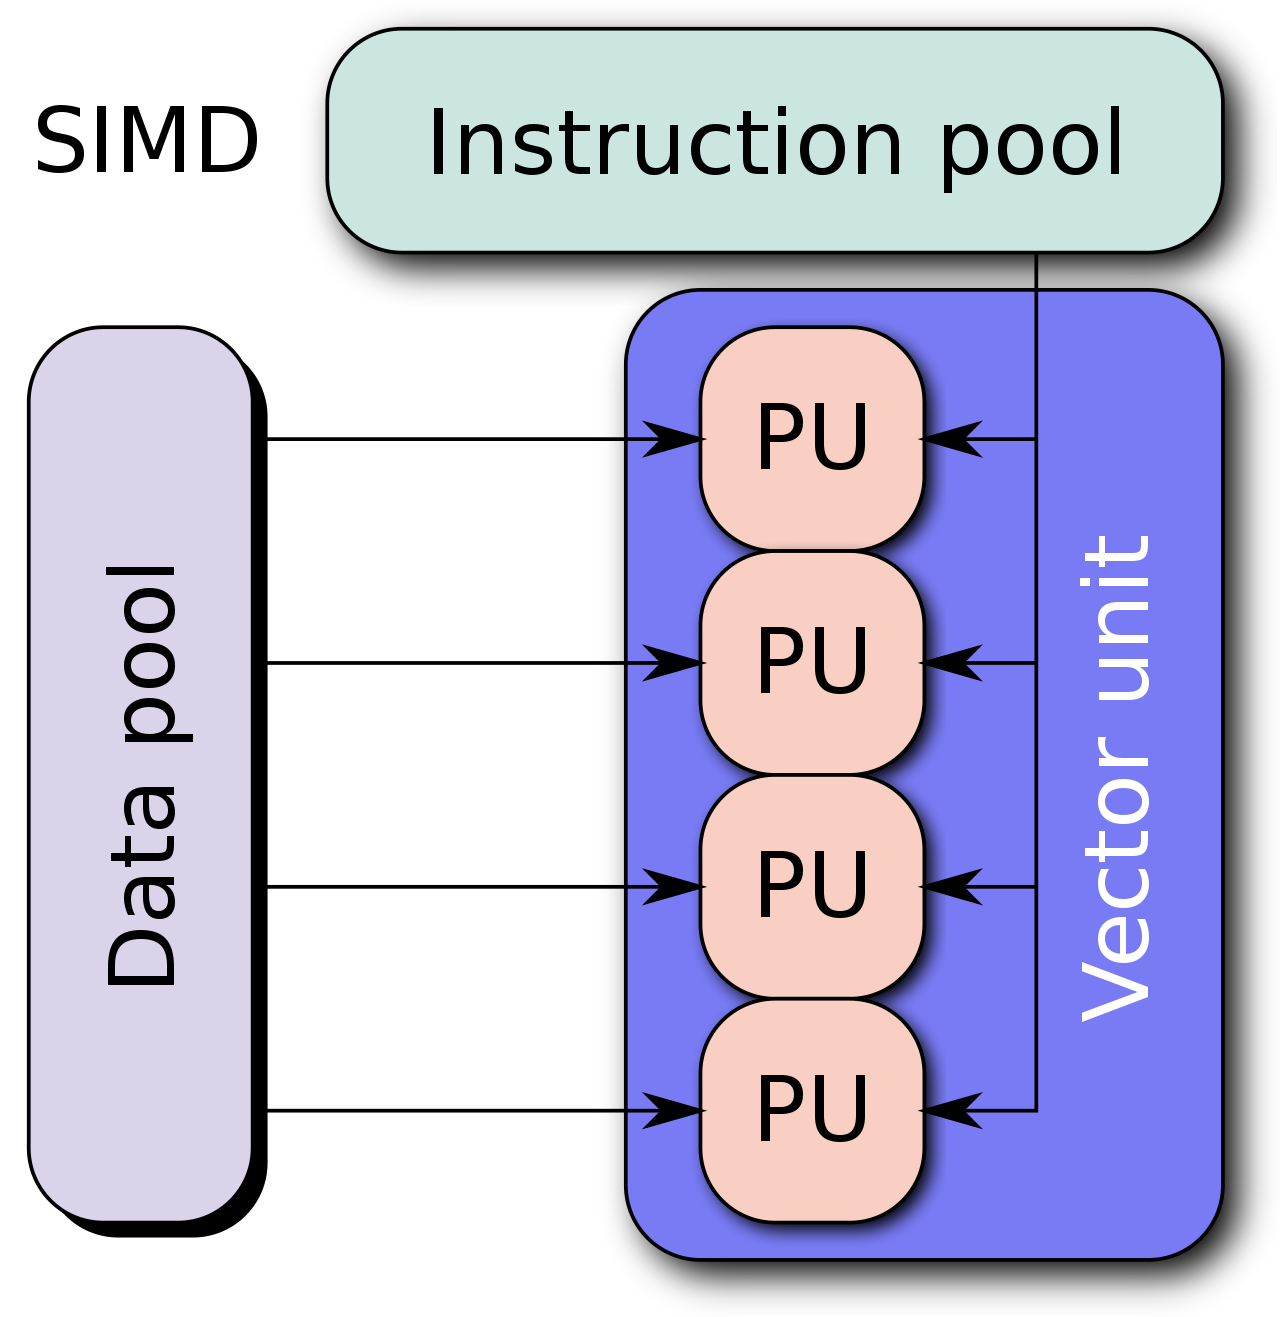
\includegraphics[height=0.5\textheight]{images/SIMD2.svg.png}
        \caption{SIMD}
    \end{figure}

\end{frame}

\begin{frame}
    \frametitle{Benefits of SIMD}

    通常情况下我们很难将串行代码转化为并行,为了设计并行算法通常需要改变原有的
    逻辑。

    \begin{figure}[h]
        \centering
        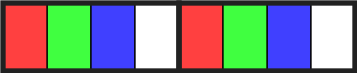
\includegraphics[width=0.5\textwidth]{images/rgba.png}
        \caption{RGBA}
    \end{figure}

    如图所示,在图形学中我们经常需要计算图像的颜色信息,而颜色在RGBA几个维度下
    的计算是可以向量化的。

\end{frame}


\begin{frame}
    \frametitle{GPGPU}

    显卡(GPU)包含大量的核心来支持高度并行化的计算,最开始的在显卡上的编程是很困
    难的,随着时代的发展显卡的计算能力越来越不容小觑,通用计算显卡(GPGPU)也开始
    包含在编译优化的领域。如何把科研大佬写的模型,放到真正的显卡上执行?

    \begin{figure}[h]
        \centering
        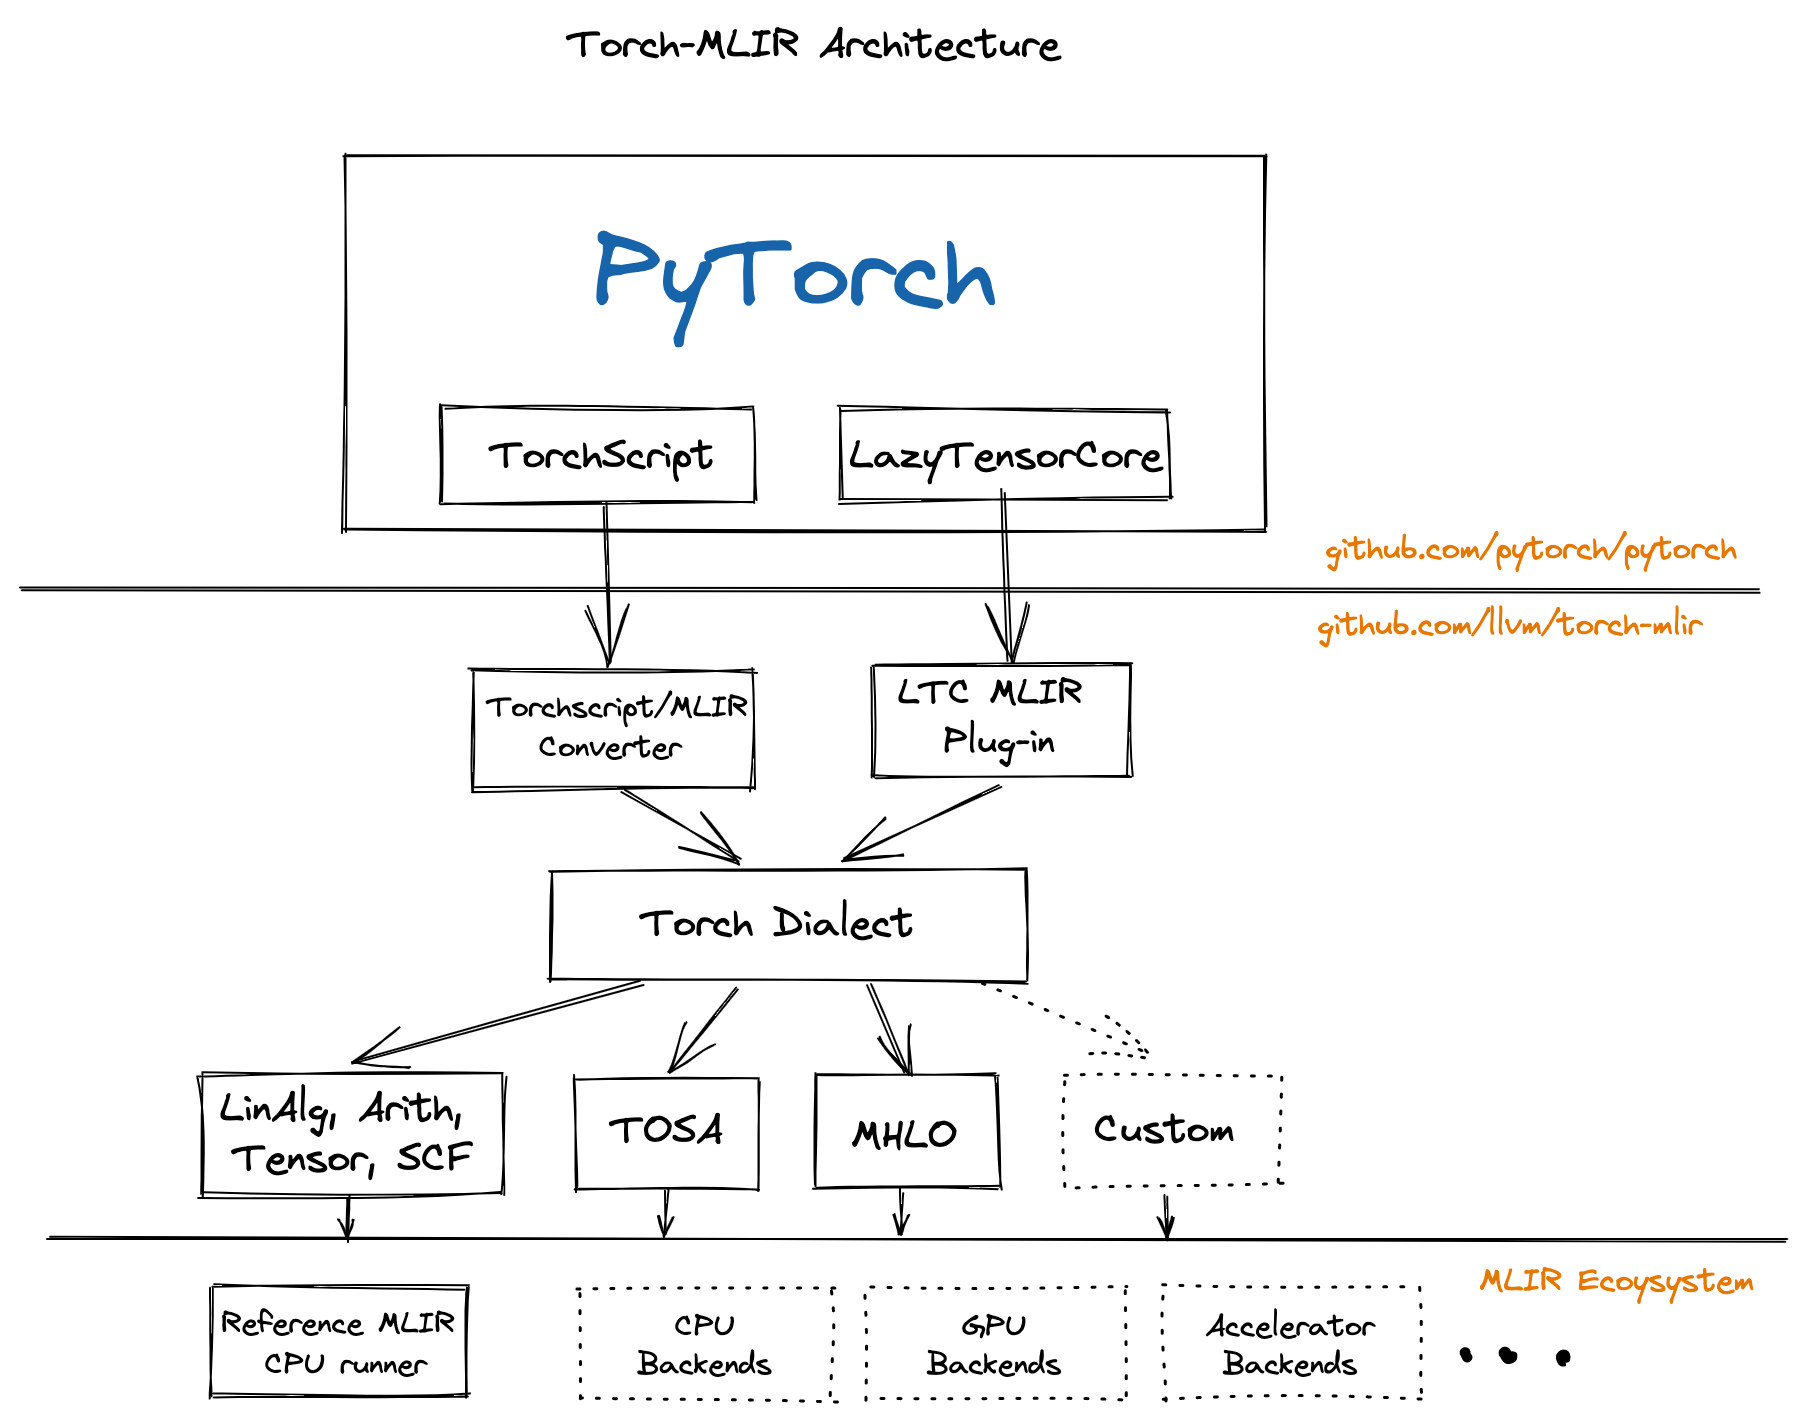
\includegraphics[height=0.5\textheight]{images/torch-mlir.png}
        \caption{Torch-MLIR}
    \end{figure}

\end{frame}

\begin{frame}
    \frametitle{Problem With SIMD Instructions}

    \begin{block}{RISC-V Designers}
        \textit{SIMD Instructions considered harmful. -- David Patterson}
    \end{block}

    一开始,SIMD被认为是实现并行化简单有效的方法。我们将64位寄存器和ALU划分为许
    多8, 16, 32位的块,然后并行地计算它们。用每条指令的操作码(opcode)提供数据宽
    度和操作。

    \textbf{指令集膨胀}

    IA-32指令集已经从最开始的80多条指令增长到了现在的1400多条。SSE, AVX, 各种
    SIMD扩展和宽寄存器让指令集变得越来越复杂。
\end{frame}

\begin{frame}[fragile]
    \frametitle{Vector vs SIMD}

    向量机与SIMD的真正区别在于,向量长度是否在机器码层面确定。

    \begin{lstlisting}
void *memcpy_vec(void *dst, void *src, size_t n) {
    void *save = dst;
    // copy data byte by byte
    for (size_t vl; n > 0; n -= vl, src += vl, dst += vl) {
        vl = vsetvl_e8m8(n);
        vuint8m8_t vec_src = vle8_v_u8m8(src, vl);
        vse8_v_u8m8(dst, vec_src, vl);
    }
    return save;
}
    \end{lstlisting}


\end{frame}

\section{Auto-Vectorization}

\begin{frame}[fragile]
    \frametitle{Auto-Vectorization}

    标量代码可以被自动向量化成含向量计算的代码。

    事实上,大量的标量循环都可以被向量化

    \begin{lstlisting}
void add(int * restrict A, int * restrict B, int n){
    for(int i = 0;i < n;i++){
        A[i] += B[i];
    }
}
    \end{lstlisting}


\end{frame}

\begin{frame}[fragile]
    \frametitle{合法性}

    数据依赖 \& Overlap (Alias Analysis)

    \begin{lstlisting}
for (int i = 0; i < N; i += 1) {
    a[i+1] = b[i] + 1;  // S1
    b[i+1] = a[i] + 1;  // S2
}
    \end{lstlisting}

    \begin{figure}
        \centering
        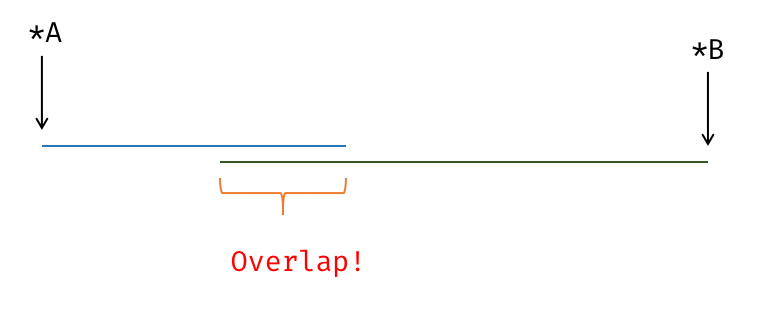
\includegraphics[width=0.4\textwidth]{images/overlap.png}
        \caption{Example of pointer overlapping}
    \end{figure}

\end{frame}

\begin{frame}
    \frametitle{收益}

    必然导致的程序大小增加 / 标量循环和向量循环的选择和跳转

    数据对齐的代价,尾循环的代价,都是需要考虑的因素。

\end{frame}

\end{document}
